\documentclass[11pt]{beamer} % mathserif for normal math fonts.
\usefonttheme[onlymath]{serif}
\usepackage[utf8]{inputenc}
\usepackage[swedish,english]{babel}
\usepackage{microtype}
\usepackage{calc}
\usepackage{amsmath,mathtools}
\usepackage[backend=biber]{biblatex}
\usepackage{contmech}
%\usepackage{subfig}
%\usepackage{movie15}
\usepackage{wasysym}
\usepackage{multimedia}
\usepackage{grffile}
\usepackage{tikz}
\usepackage{siunitx}
\usepackage{booktabs}

\usepackage{pgfplots}
\pgfplotsset{compat=1.8}
\usetikzlibrary{shapes,arrows}

\newcommand{\highlight}[1]{{\color{red}#1}}
\newcommand{\downlight}[1]{{\color{gray}#1}}
\DeclarePairedDelimiter{\homgen}{\langle}{\rangle_\rve}
\DeclarePairedDelimiter{\shomgen}{\langle\!\langle}{\rangle\!\rangle_\rve}
\DeclarePairedDelimiter{\jmp}{[\![}{]\!]}
\newcommand{\jump}[1]{[\![#1]\!]}
\newcommand{\prescribed}{\mathrm{pre}}
\newcommand{\on}{\quad\text{ on }}
\renewcommand{\dev}{\mathrm{d}}
\renewcommand{\vol}{\mathrm{v}}
\newcommand{\per}{\mathrm{per}}
\newcommand{\volume}{|\Omega_\rve|}
\newcommand{\ded}{\mathrm{d}}
\newcommand{\dep}{\mathrm{p}}
\newcommand{\Periodic}{\mathrm{P}}
\newcommand{\external}{\mathrm{ext}}
\newcommand{\surf}{\mathrm{s}}
\newcommand{\pore}{\mathrm{pore}}
\newcommand{\particle}{\mathrm{part}}
\newcommand{\devop}{\ts\epsilon_\dev}
\newcommand{\densinv}{\eta}
\newcommand{\dens}{\eta^{-1}}
\newcommand{\epspargs}{\{{\bar{\ts d}}_\dev, \bar{p}\}}
\newcommand{\rve}{
  {\mathchoice
   {\mbox{\scalebox{0.67}{$\Box$}}}
   {\mbox{\scalebox{0.67}{$\Box$}}}
   {\mbox{\scalebox{0.5}{$\Box$}}}
   {\mbox{\scalebox{0.375}{$\Box$}}}
  }
}
\newcommand{\Co}{\mathrm{Co}}
\newcommand{\WC}{\mathrm{WC}}
\newcommand{\yield}{\mathrm{y}}
\newcommand{\hyd}{\mathrm{hyd}}
\newcommand{\elast}{\mathrm{elast}}
\newcommand{\eq}{\mathrm{V}}
%\usepgfplotslibrary{patchplots}
%\usepgfplotslibrary{groupplots}
%\pgfplotsset{compat=1.3}

\newcommand{\roughcite}[1]{\textsc{#1}}
\renewcommand{\alert}[1]{\textbf{#1}}

\setbeamersize{text margin left=.3cm,text margin right=.3cm}

\usetheme[titleflower=false]{chalmers}
\title{
Mesoscale modeling of hardmetal
}
\author[Mikael \"Ohman COMPLAS XIII  --- 2015-09-03]{Mikael \"Ohman\textsuperscript{*}\\Sven Johansson\textsuperscript{\dag}\\Göran Wahnstr\"om\textsuperscript{\dag}\\Magnus Ekh\textsuperscript{*}\\Fredrik Larsson\textsuperscript{*}\\Kenneth Runesson\textsuperscript{*}}
\institute{Department of Applied Mechanics\textsuperscript{*}\\Department of Applied Physics\textsuperscript{\dag}\\Chalmers University of Technology\\
mikael.ohman@chalmers.se
}
%\titlepageextra{2012}% session: Multiple-scale physics and computation
\date{2015-09-03}
%\footer{\insertshortauthor\ 2\textsuperscript{nd} ICMM}
\titlepagelogofile{Avancez_gold}

% Bibliography
%\bibliography{references_extended}

% Speeds up compilation.
% \usetikzlibrary{external}
% \tikzexternalize


\addbibresource{Multiscale.bib}

\begin{document}

\section{Title page}
\begin{frame}[plain]
 \titlepage
\end{frame}


\section{Outline}
%%%%%%%%%%%%%%%%%%%%%%%%%%%%%%%%%%%%%%%%%%%%%%%%%%%%%%%%%%%%%%%%%%%%%%%%%%%%%%%%%%%%%%%%%%%%%%%%%%%
\begin{frame}
 \frametitle{Outline}
\begin{itemize}
 \item Background
 \item WC-Co grain-structures --- characteristics and numerical generation
 \item Modeling of WC and Co
 \item Numerical examples
\end{itemize}
\end{frame}


\section{Background}
%%%%%%%%%%%%%%%%%%%%%%%%%%%%%%%%%%%%%%%%%%%%%%%%%%%%%%%%%%%%%%%%%%%%%%%%%%%%%%%%%%%%%%%%%%%%%%%%%%%
\begin{frame}
 \frametitle{Background}
  \begin{itemize}
    \item Why investigate WC-Co microstructures?
    \begin{itemize}
      \item WC-Co systems --- an important class of hardmetals
      \item Extreme loads at high temperatures (machining tools)
      \item GPa-magnitude of residual stresses during manufacturing
      \item Grain structure heavily influences strength
    \end{itemize}
  \end{itemize}
  \begin{center}
   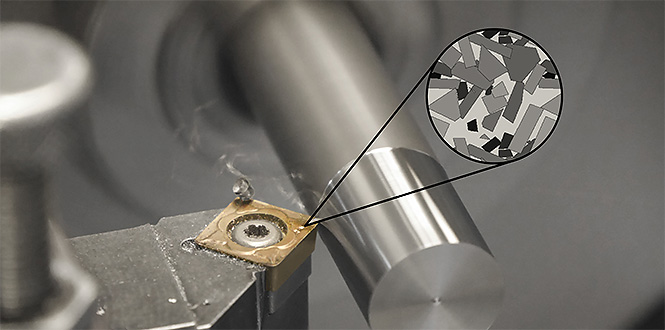
\includegraphics[width=0.8\linewidth]{figures/cutting_tool_and_microstruct_big}
  \end{center}
\end{frame}


\section{Grain structure}
%%%%%%%%%%%%%%%%%%%%%%%%%%%%%%%%%%%%%%%%%%%%%%%%%%%%%%%%%%%%%%%%%%%%%%%%%%%%%%%%%%%%%%%%%%%%%%%%%%%
\begin{frame}
 \frametitle{WC-Co grain structures}
  \begin{itemize}
  \item 10-20 \% Co by volume
  \item WC: HCP-crystal structure
  \item Co: FCC-crystal structure
  \item Thin layers of Co between WC-grains
  \item Need something better than voronoi tesselation in order to capture the characteristics of WC-Co
  \end{itemize}
  \begin{center}
   \begin{tikzpicture}
    \node at (0,0) {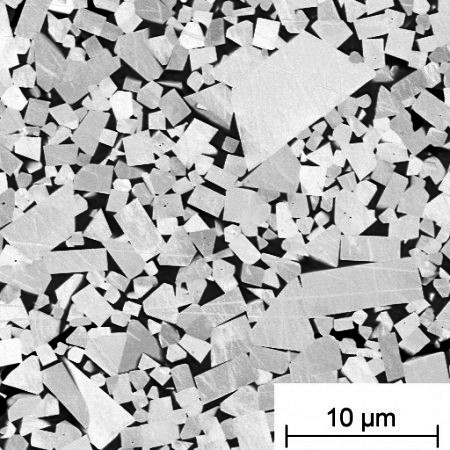
\includegraphics[width=0.3\linewidth]{figures/WC-Co}};
    \node at (2.5cm, 0) {$\quad\neq\quad$};
    \node at (5cm, 0) {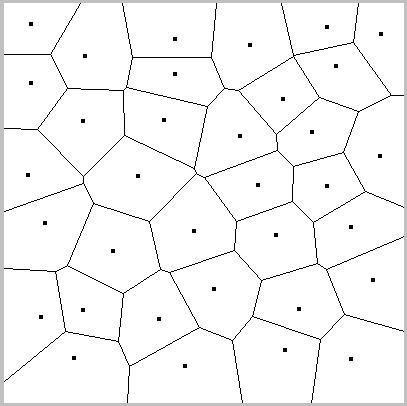
\includegraphics[width=0.3\linewidth]{figures/voronoi}};
   \end{tikzpicture}
  \end{center}
\end{frame}


%%%%%%%%%%%%%%%%%%%%%%%%%%%%%%%%%%%%%%%%%%%%%%%%%%%%%%%%%%%%%%%%%%%%%%%%%%%%%%%%%%%%%%%%%%%%%%%%%%%
\begin{frame}
 \frametitle{WC grains}
  \begin{itemize}
  \item Randomly oriented grains in Co-matrix
  \item Ideal shape; truncated prisms
  \begin{center}
    \raisebox{-0.5\height}{
    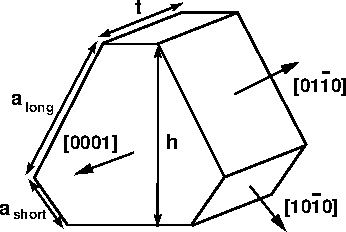
\includegraphics[width=.3\linewidth]{figures/tt_drawing}
    }
    \raisebox{-0.5\height}{
    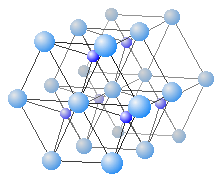
\includegraphics[width=.3\linewidth]{figures/WC_atoms}
    }
  \end{center}
  \item Dimensions are controlled by various additives in the WC-Co mixture.
  \item $\Sigma2$ interfaces common within grains (not presently included)
  \end{itemize}
\end{frame}

%%%%%%%%%%%%%%%%%%%%%%%%%%%%%%%%%%%%%%%%%%%%%%%%%%%%%%%%%%%%%%%%%%%%%%%%%%%%%%%%%%%%%%%%%%%%%%%%%%%
\begin{frame}
 \frametitle{Generating WC-Co grain-structures}
  \begin{itemize}
  \item Need to identify individual WC grains (limitation of \textsc{Magin and Gerard (2009), Digimat}) due to anisotropy and inter-grain sliding
  \item Inter-grain surfaces are complex in 3D $\implies$ CAD-based descriptions are difficult to work with.
  \item Voxel based description used:
   \begin{itemize}
    \item[+] Same format as experimental data (``slice and view'')
    \item[+] Very flexible
    \item[+] Quite fast
    \item[-] Requires complex surface reconstruction for interfaces
   \end{itemize}
   \item CCBuilder (Compacted Carbide Builder): Open source tool developed for generating microstructures
    \begin{itemize}
     \item Generates realistic WC-Co microstructures
     \item Targets important statistical measurements and distributions
     \item Written in Python+Cython
    \end{itemize}
  \end{itemize}
\end{frame}


%%%%%%%%%%%%%%%%%%%%%%%%%%%%%%%%%%%%%%%%%%%%%%%%%%%%%%%%%%%%%%%%%%%%%%%%%%%%%%%%%%%%%%%%%%%%%%%%%%%
\begin{frame}
 \frametitle{CCBuilder: Capturing microstructure characteristics}
 \begin{columns}
 \column{.5\textwidth}
  \begin{itemize}
  \item Input
   \begin{itemize} 
    \item Desired volume fraction 
    \item Grain size distribution
    \item RVE-size
    \item Voxel discretization
   \end{itemize}
  \item Grains inserted with random orientation
  \item Various techniques for grain placement
  \item Analysis files exported to OOFEM using Voxels as hexahedral finite elements
  \end{itemize}
 \column{.5\textwidth}
 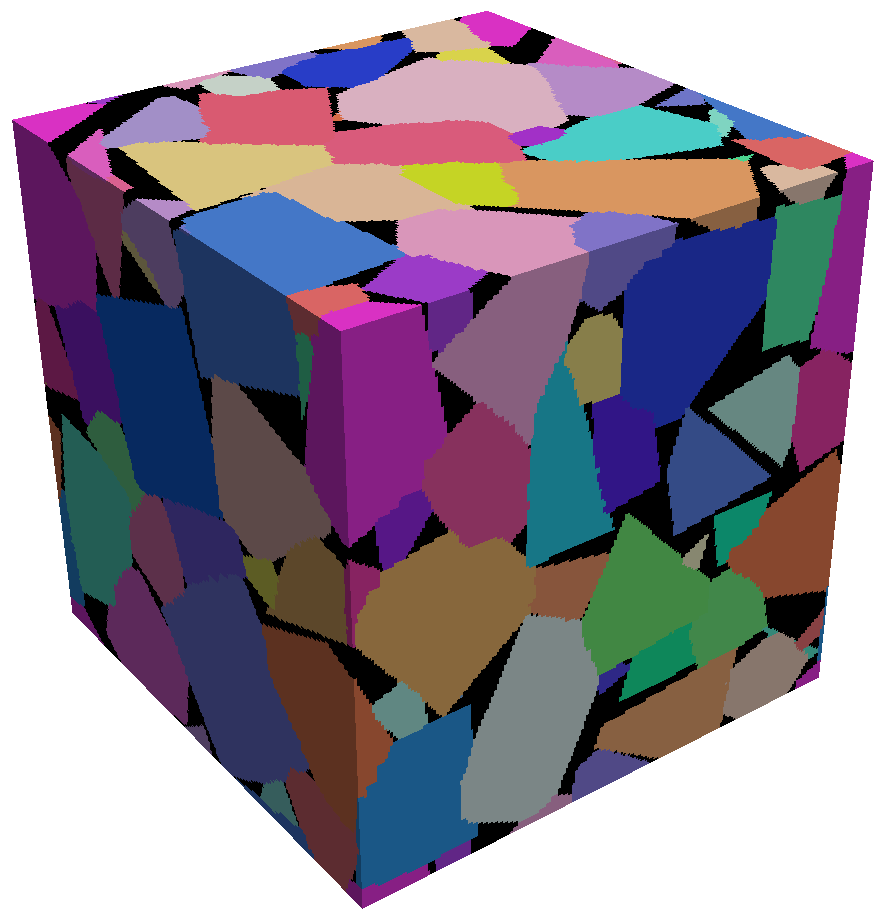
\includegraphics[width=1\linewidth]{3D_view_e}
  \end{columns}
\end{frame}

%%%%%%%%%%%%%%%%%%%%%%%%%%%%%%%%%%%%%%%%%%%%%%%%%%%%%%%%%%%%%%%%%%%%%%%%%%%%%%%%%%%%%%%%%%%%%%%%%%%
\begin{frame}
 \frametitle{Potts simulation}
  \begin{itemize}
   \item Stochastic simulation dealing with overlapping regions (minizes grain-grain surfaces)
   \item More realistic grain shapes
   \item Slightly improve contiguity
  \end{itemize}
  \begin{center}
   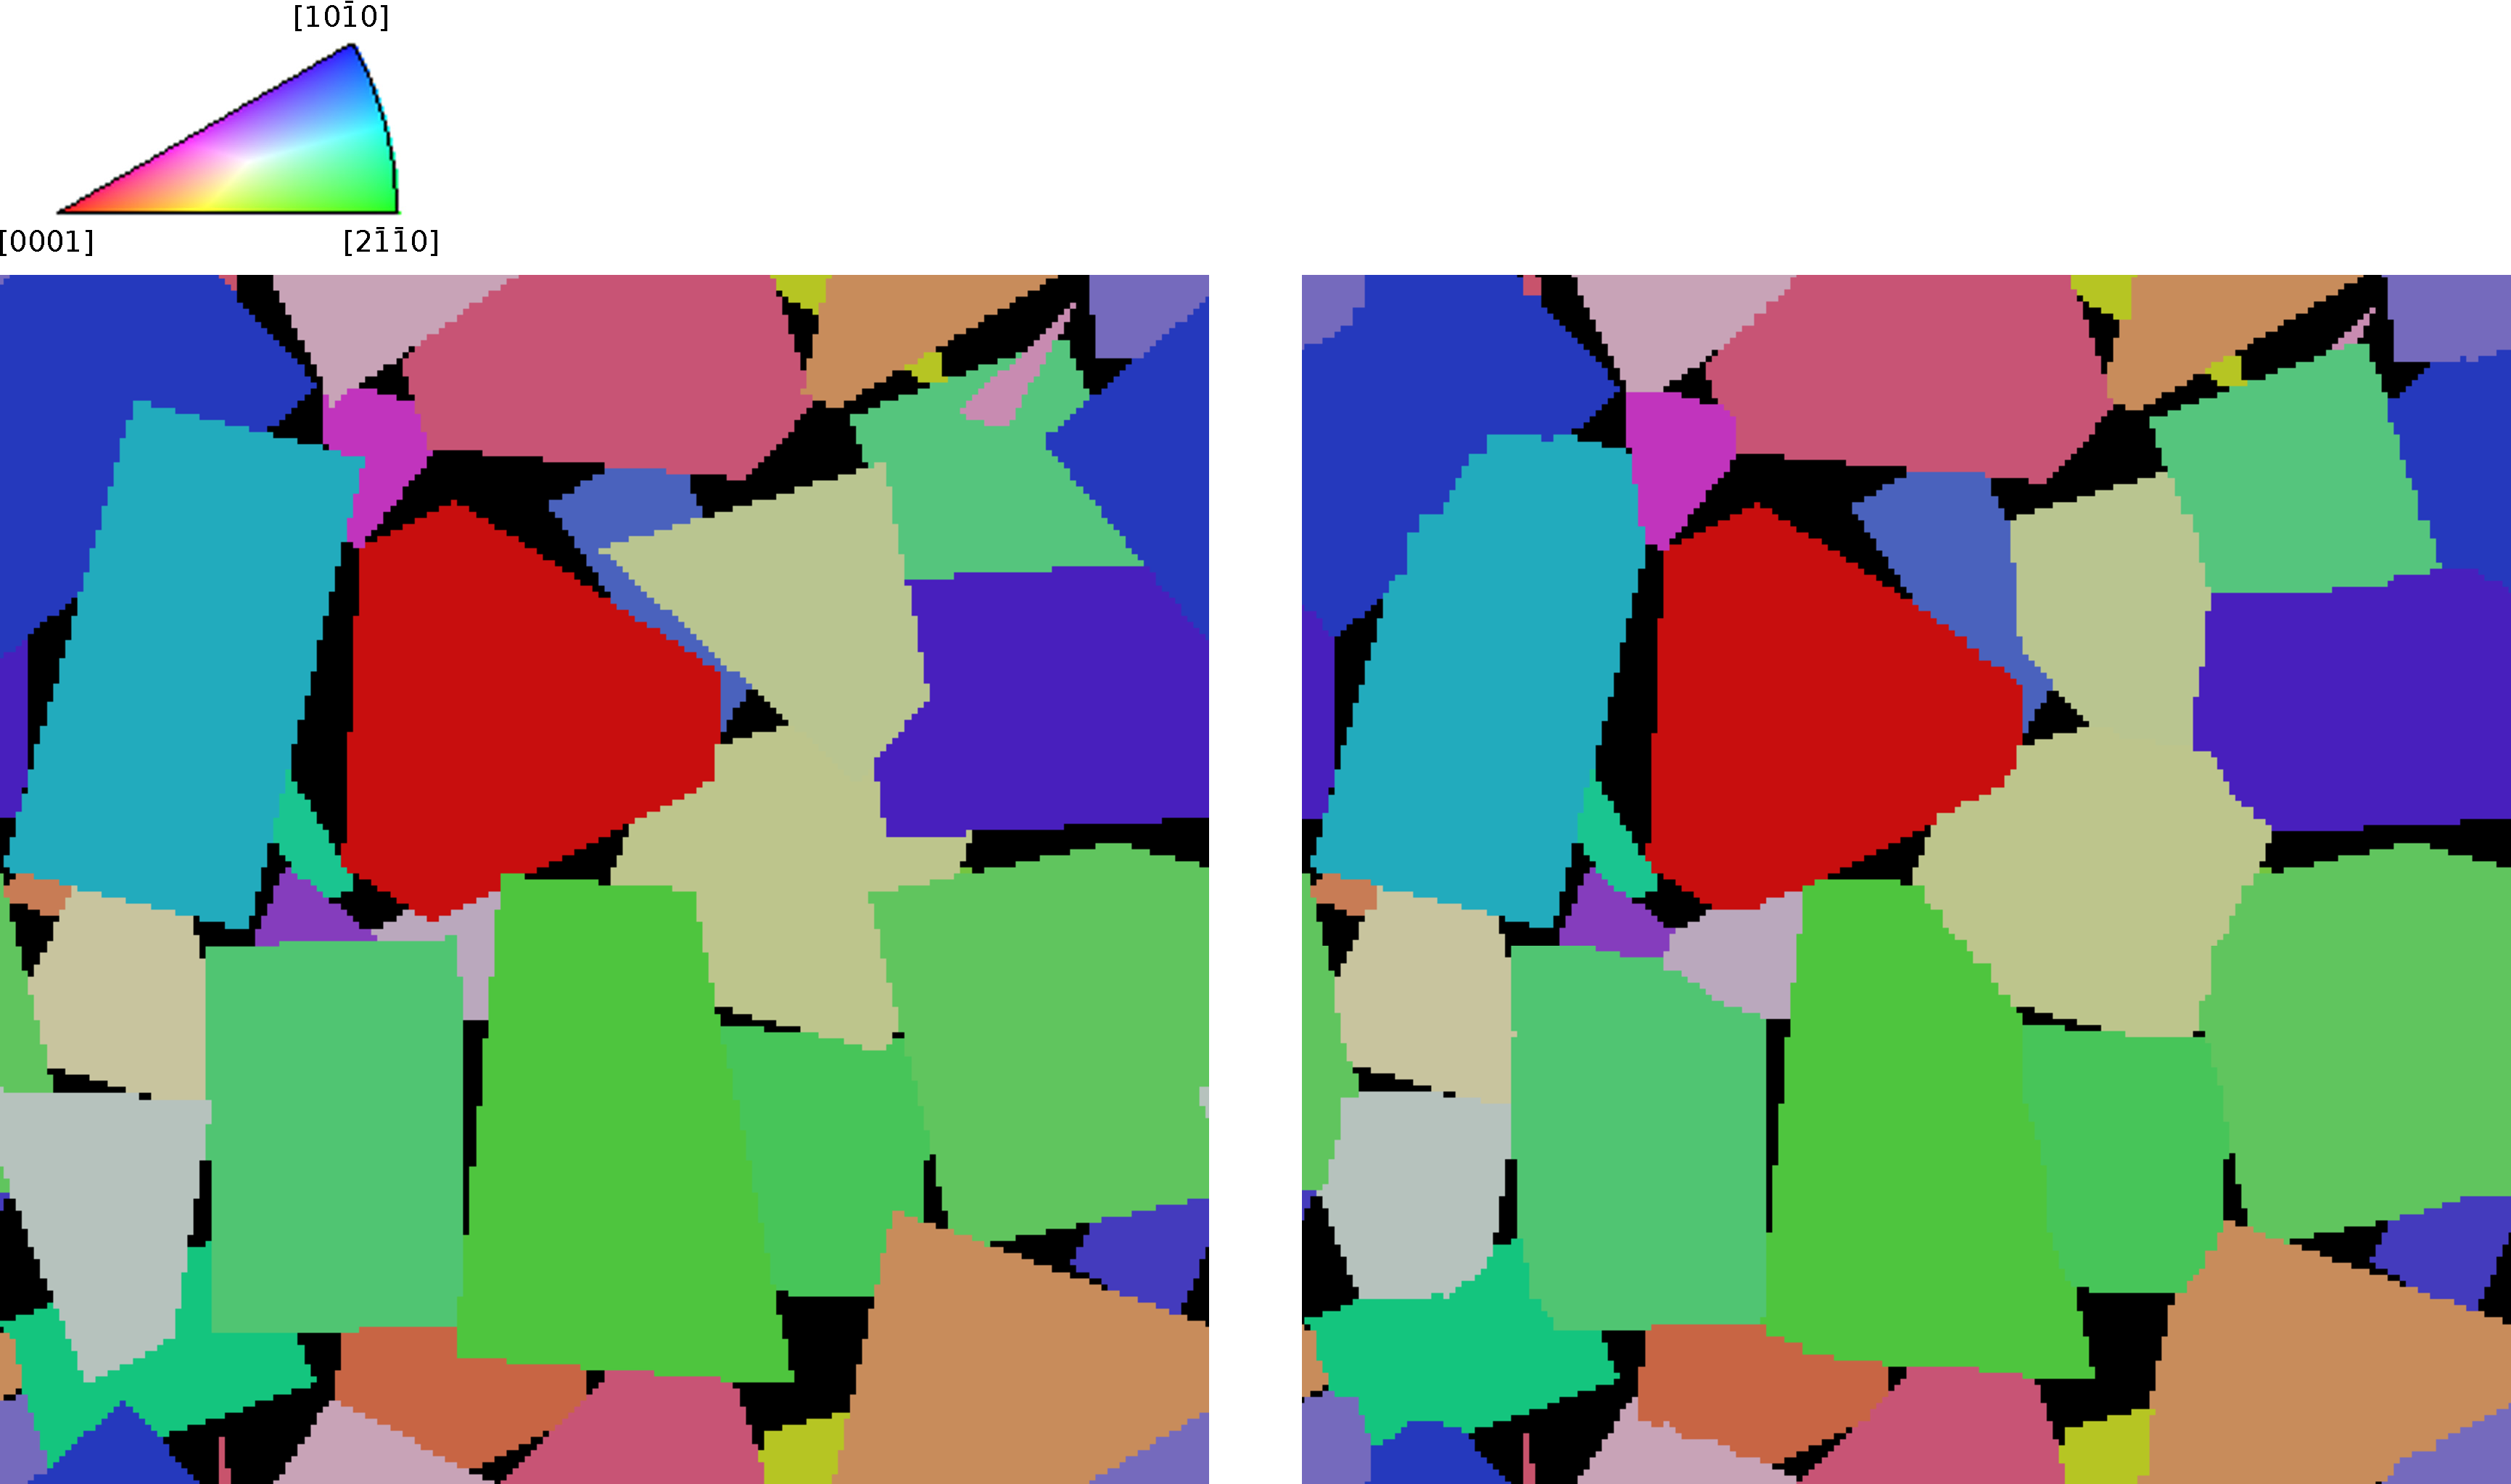
\includegraphics[trim=0 0 0 6cm,clip, width=0.9\linewidth]{v105_slice1}
  \end{center}
\end{frame}


%%%%%%%%%%%%%%%%%%%%%%%%%%%%%%%%%%%%%%%%%%%%%%%%%%%%%%%%%%%%%%%%%%%%%%%%%%%%%%%%%%%%%%%%%%%%%%%%%%%
\begin{frame}
 \frametitle{Contiguity}
  \begin{itemize}
   \item Contiguity $ C \defeq 2 A_{WC-WC} / ( 2 A_{WC-WC} + A_{WC-Co} )$ (grain-grain surface fraction) is frequently documented in literature
   \item Strategy for placing grains is important to match
   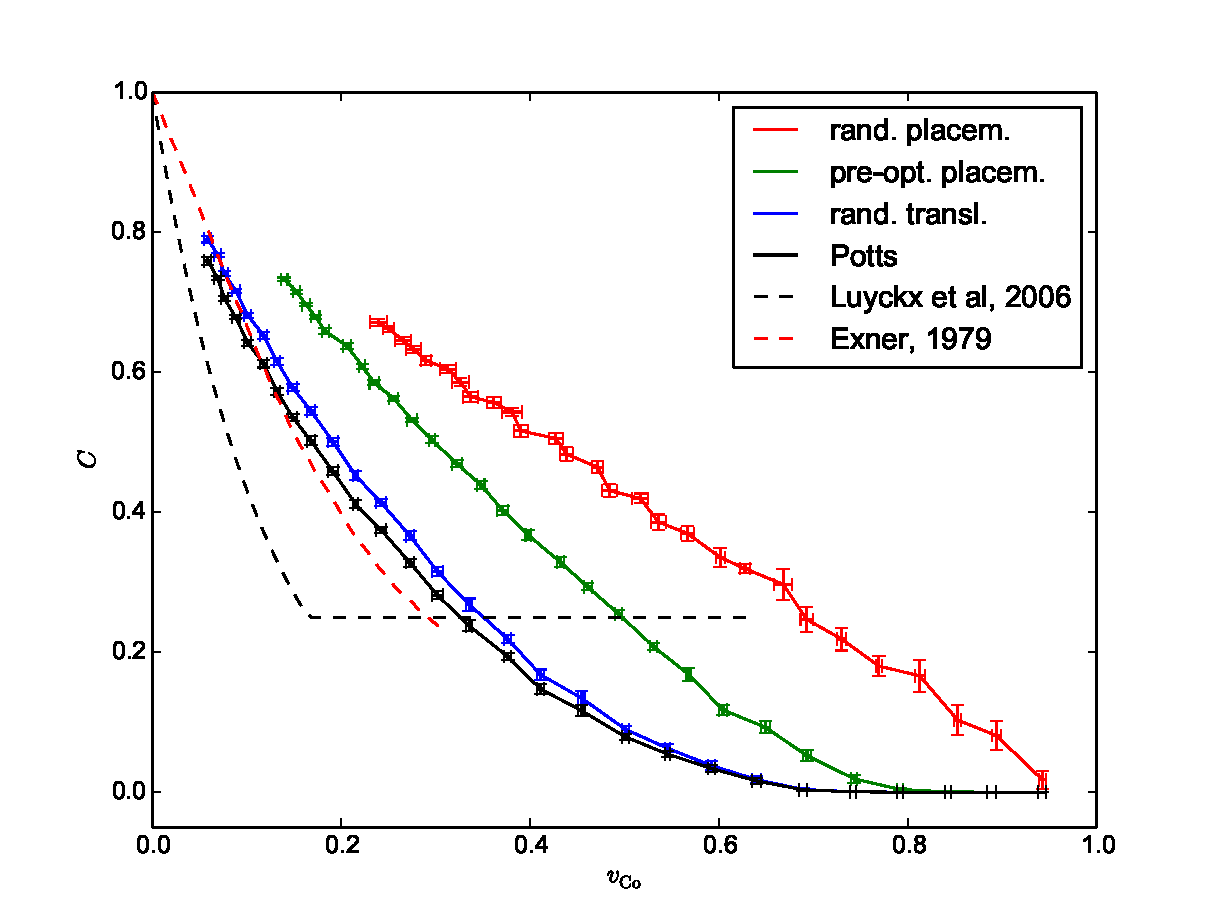
\includegraphics[width=0.75\linewidth]{contiguity}
  \end{itemize}
\end{frame}


%%%%%%%%%%%%%%%%%%%%%%%%%%%%%%%%%%%%%%%%%%%%%%%%%%%%%%%%%%%%%%%%%%%%%%%%%%%%%%%%%%%%%%%%%%%%%%%%%%%
\begin{frame}
 \frametitle{Misorientation distribution}
  \begin{itemize}
   \item Measurements of the relative orientation of grains
   \item Tests with large RVEs ($\approx$4k grains, $\approx$23k grain-grain contacts)
   \item Good fit with theoretical distribution for randomly oriented particles.
   \item Indicates that no artificial anisotropy has been induced by the non-random grain placement.
  \end{itemize}
  \begin{center}
   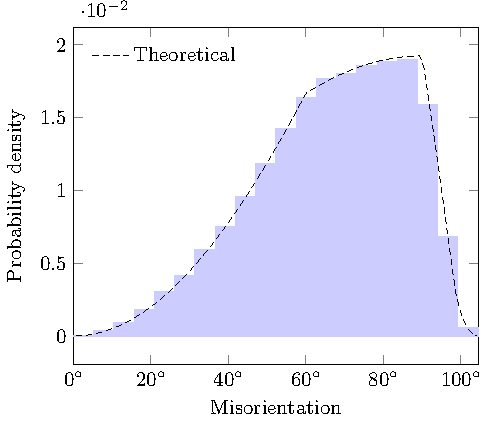
\includegraphics[scale=0.7]{WCResidualStress-figure1}
   %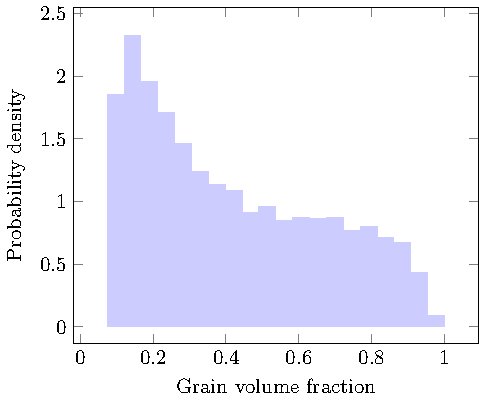
\includegraphics[scale=0.7]{WCResidualStress-figure2}
  \end{center}
\end{frame}


\section{Modeling}
%%%%%%%%%%%%%%%%%%%%%%%%%%%%%%%%%%%%%%%%%%%%%%%%%%%%%%%%%%%%%%%%%%%%%%%%%%%%%%%%%%%%%%%%%%%%%%%%%%%
\begin{frame}
 \frametitle{WC grains}
  \begin{itemize}
  \item HCP $\implies$ transversely isotropic elastic and thermal coefficients
  \begin{align*}
   \ts{C} = \begin{pmatrix} C_{11} & C_{12} & C_{13} & 0 & 0 & 0 \\
                                C_{12} & C_{11} & C_{13} & 0 & 0 & 0 \\
                                C_{13} & C_{13} & C_{33} & 0 & 0 & 0 \\
                                0 & 0 & 0 & C_{44} & 0 & 0 \\
                                0 & 0 & 0 & 0 & C_{44} & 0 \\
                                0 & 0 & 0 & 0 & 0 & C_{66} \\
                \end{pmatrix}, \quad
    \ts{\alpha} = \begin{pmatrix} \alpha_{11} \\ \alpha_{11} \\ \alpha_{33} \\ 0 \\ 0 \\ 0 \end{pmatrix}
  \end{align*}
  \begin{align*}
    \ts\sigma = \ts C \cdot (\ts\epsilon - \ts\alpha \, \Delta T)
  \end{align*}
  \item Coefficients are well documented \textsc{Lee \& Gilmore (1982)}
  \begin{align*}
     C_{11} &= 720\si{\giga\pascal},\; C_{12} = 254\si{\giga\pascal},\; C_{13} = 267\si{\giga\pascal}, \\
     C_{33} &= 972\si{\giga\pascal},\; C_{44} = 328\si{\giga\pascal},\; C_{66} = \frac12 (C_{11}-C_{12})
     \\
     \alpha_1 &= \num{5.2e-6},\; \alpha_3 = \num{7.3e-6}
  \end{align*}
  \end{itemize}
\end{frame}

%%%%%%%%%%%%%%%%%%%%%%%%%%%%%%%%%%%%%%%%%%%%%%%%%%%%%%%%%%%%%%%%%%%%%%%%%%%%%%%%%%%%%%%%%%%%%%%%%%%
\begin{frame}
 \frametitle{Co matrix}
  \begin{itemize}
  \item FCC-crystal structure: Isotropic elasticity.
  \item Isotropic, $E = 211\si{\giga\pascal}$, $\nu = 0.31$, $\alpha = \num{13.8e-5}$.
  \item Plastic behavior difficult to ascertain
   \begin{itemize}
    \item Varying diffusion of C in Co matrix
    \item Temperature dependent
    \item Few experimental results on pure Co
    \item Yield stress \SIrange{250}{600}{\mega\pascal} at room temperature
    \item Hardening ?
   \end{itemize}
  \end{itemize}
\end{frame}

\subsection{Residual stress}
%%%%%%%%%%%%%%%%%%%%%%%%%%%%%%%%%%%%%%%%%%%%%%%%%%%%%%%%%%%%%%%%%%%%%%%%%%%%%%%%%%%%%%%%%%%%%%%%%%%
\begin{frame}
 \frametitle{Residual thermal stress analysis}
 \begin{columns}
 \column{0.5\textwidth}
 \begin{itemize}
  \item Experiments suggest stress buildup starting at +800\si{\kelvin},\\ \textsc{D. Mari et al. (2009)}
  \item Cooling in free sintering $\implies$ zero macroscopic stress: $\bar{\ts\sigma} = \ts 0$

  \item Using RVE consisting of 165 grains, with $10^6$ elements
  \item Standard homogenization with periodic boundary conditions
 \end{itemize}
 \column{0.5\textwidth}
 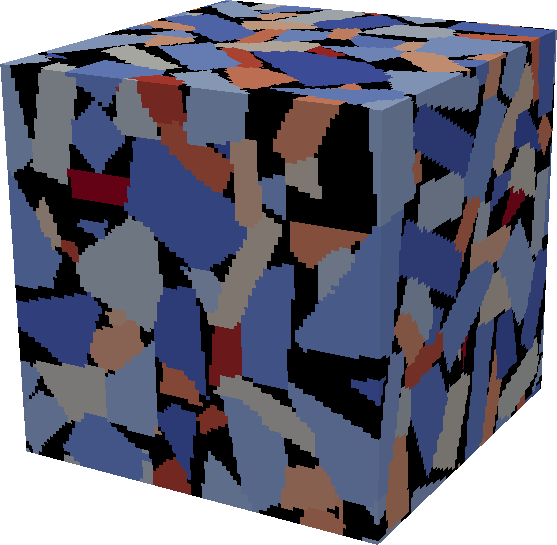
\includegraphics[width=1\linewidth]{figures/RVE}
 \end{columns}
\end{frame}

%%%%%%%%%%%%%%%%%%%%%%%%%%%%%%%%%%%%%%%%%%%%%%%%%%%%%%%%%%%%%%%%%%%%%%%%%%%%%%%%%%%%%%%%%%%%%%%%%%%
\begin{frame}
 \frametitle{Numerical example: Influence of Co phase modeling}
 \begin{figure}[htbp!]
 \centering
  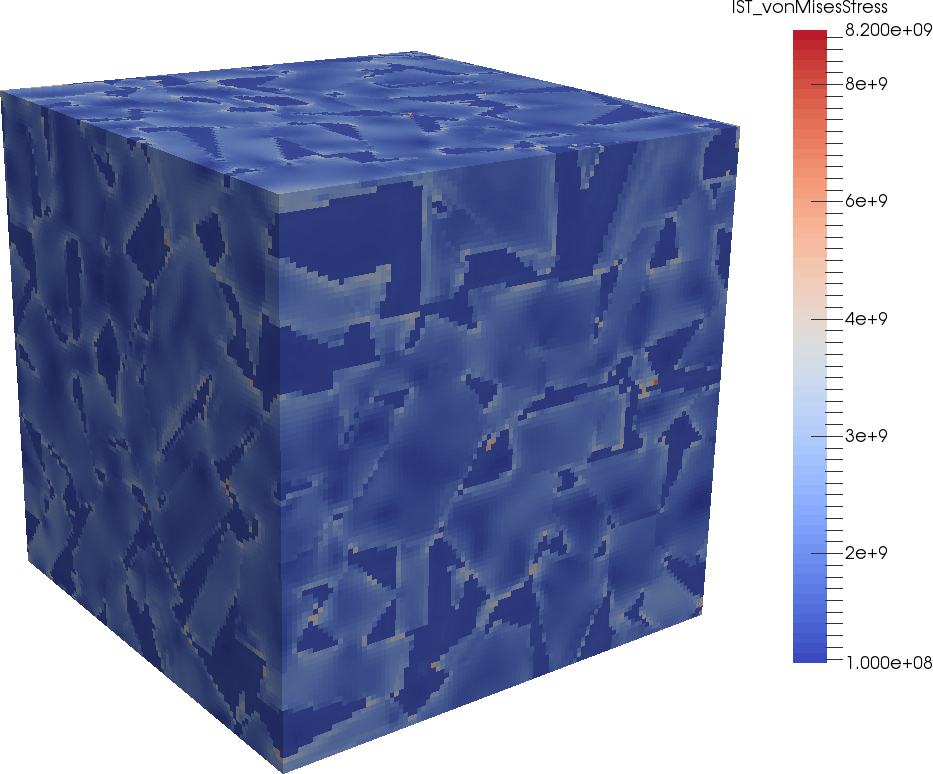
\includegraphics[scale=0.20]{rve_vonmises}
  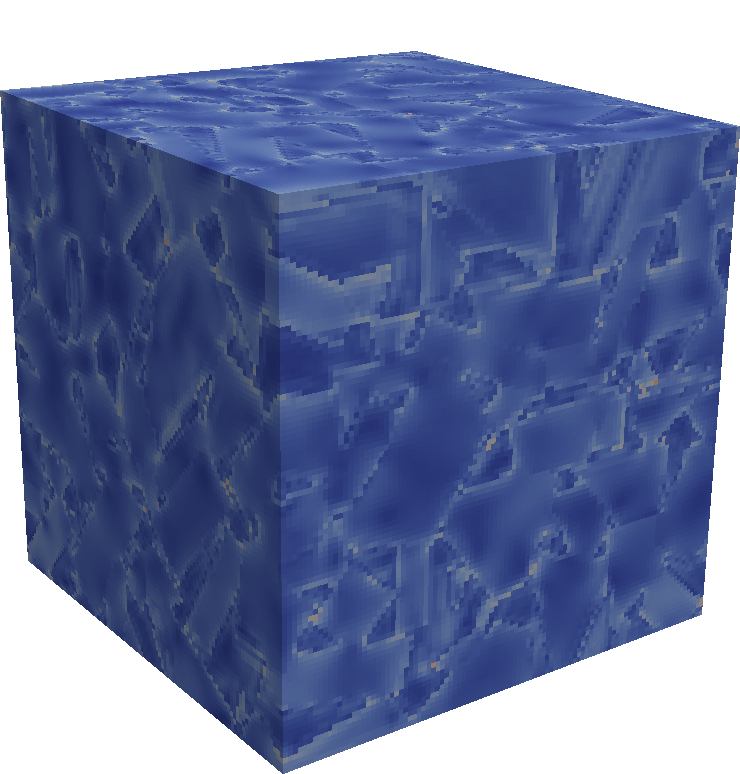
\includegraphics[scale=0.20]{rve_vonmises_elastic}
 \caption{Comparison of von-Mises stress distribution with elasto-plastic (left) and elastic (right) cobalt phase} \label{fig:rve_stress}
\end{figure}
\end{frame}



%%%%%%%%%%%%%%%%%%%%%%%%%%%%%%%%%%%%%%%%%%%%%%%%%%%%%%%%%%%%%%%%%%%%%%%%%%%%%%%%%%%%%%%%%%%%%%%%%%%
\begin{frame}
 \frametitle{Stress distribution}
  \begin{itemize}
   \item \small Elastolastic Co\hfill
   \raisebox{-0.5\height}{
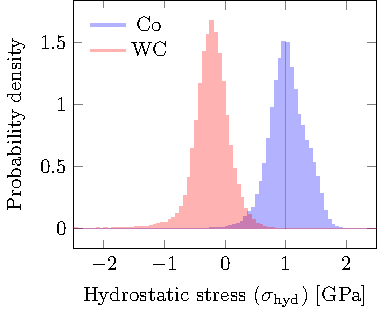
\includegraphics[scale=0.7]{WCResidualStress-figure3}
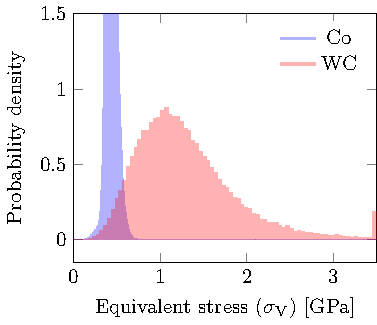
\includegraphics[scale=0.7]{WCResidualStress-figure4}
}
\item Elastic Co\hfill
   \raisebox{-0.5\height}{
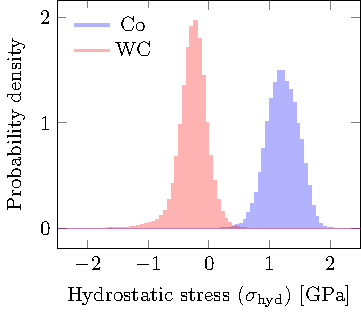
\includegraphics[scale=0.7]{WCResidualStress-figure5}
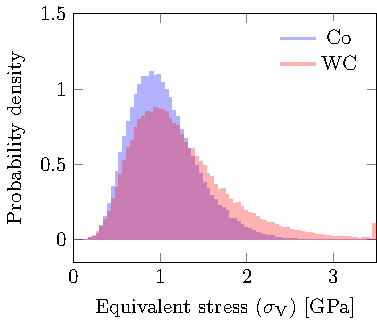
\includegraphics[scale=0.7]{WCResidualStress-figure6}
}
  \end{itemize}
\end{frame}

%%%%%%%%%%%%%%%%%%%%%%%%%%%%%%%%%%%%%%%%%%%%%%%%%%%%%%%%%%%%%%%%%%%%%%%%%%%%%%%%%%%%%%%%%%%%%%%%%%%
\begin{frame}
 \frametitle{Comparison of stresses}
  \begin{itemize}
  \item 2D analysis by Exnar et al.
  \item Neutron diffraction experiments from Mari et al. 
  \item More data available in literature with a fairly large spread of values
  \item Average and variance in each phase:
 \end{itemize}
\begin{center}
\begin{tabular}{l|r|r||r|r}
                           & Plastic Co & Elastic Co & Mari et al. & Exnar et al.\\
                           \midrule
 $\bar{\sigma}_{\WC,\hyd}$ & $ -222 \pm 513 $          & $ -262 \pm 473 $ & $ -400 $ & $ -210\pm110 $\\
 $\bar{\sigma}_{\Co,\hyd}$ & $ 1030 \pm 816 $          & $ 1216 \pm 948 $ & $ 1847 $ & $ 1330\pm150 $\\
 $\bar{\sigma}_{\WC,\eq}$  & $ 1301 \pm 595 $          & $ 1234 \pm 573 $ &          & $  700\pm320 $\\
 $\bar{\sigma}_{\Co,\eq}$  & $ 430 \pm \phantom{0}54 $ & $ 1043 \pm 385 $ &          & $  950\pm480 $\\
\end{tabular}
 \end{center}
\end{frame}


\section{End}
%%%%%%%%%%%%%%%%%%%%%%%%%%%%%%%%%%%%%%%%%%%%%%%%%%%%%%%%%%%%%%%%%%%%%%%%%%%%%%%%%%%%%%%%%%%%%%%%%%%
\begin{frame}
 \frametitle{Conclusions and future work}
 \begin{itemize}
 \item Residual stresses in agreement with values found in literature
 \item \texttt{CCBuilder} and \texttt{OOFEM} on GitHub.
 \end{itemize}

  \begin{itemize}
  %\item Absolute grain sizes should influence macroscopic strength (\textsc{Coats et al.\ (2003)})
  \item Cohesive zone modeling: Requires smooth surface reconstruction
  \item Crystal plasticity
  \item Material data from molecular dynamics simulations combined with experiments
 \end{itemize}

\end{frame}

\end{document}
